\documentclass{article}
% ~ ~ ~ ~ ~ ~ ~ ~ ~ ~ ~ ~ ~ ~ ~ ~ ~ ~ ~ ~ ~ ~ ~ ~ ~ ~ ~ ~ ~ ~ ~ ~ ~ ~ ~ ~ ~ ~ ~ ~ ~ ~ ~ ~ ~ ~ ~ ~

\usepackage[utf8]{inputenc}
\usepackage{amsmath}
\usepackage{amssymb} % for \mathbb
\usepackage{graphicx} % for figures
\usepackage{color}
\usepackage[usenames,dvipsnames]{xcolor}
\usepackage{hyperref} % for hyperlinks
\usepackage{float} % for figures
% ~ ~ ~ ~ ~ ~ ~ ~ ~ ~ ~ ~ ~ ~ ~ ~ ~ ~ ~ ~ ~ ~ ~ ~ ~ ~ ~ ~ ~ ~ ~ ~ ~ ~ ~ ~ ~ ~ ~ ~ ~ ~ ~ ~ ~ ~ ~ ~
% CUSTOM COLOUR
\definecolor{DGrey}{rgb}{0.1,0.1,0.1} % Dark Grey
% ~ ~ ~ ~ ~ ~ ~ ~ ~ ~ ~ ~ ~ ~ ~ ~ ~ ~ ~ ~ ~ ~ ~ ~ ~ ~ ~ ~ ~ ~ ~ ~ ~ ~ ~ ~ ~ ~ ~ ~ ~ ~ ~ ~ ~ ~ ~ ~
\title{ Introduction to Engineering Written Assignment Questions}
\date{January 2013}
\author{Greg Mayer and Daniel Connelly}
% ~ ~ ~ ~ ~ ~ ~ ~ ~ ~ ~ ~ ~ ~ ~ ~ ~ ~ ~ ~ ~ ~ ~ ~ ~ ~ ~ ~ ~ ~ ~ ~ ~ ~ ~ ~ ~ ~ ~ ~ ~ ~ ~ ~ ~ ~ ~ ~
% HEADER/FOOTER
\usepackage{fancyheadings}
\pagestyle{myheadings} % set headings to be user defined
\fancyhead{} % To create custom header, clear default layout
\renewcommand{\subsectionmark}[1]{\markright{{\color{DGrey}\thesubsection} \ {\color{DGrey}#1}}}
\fancyhead[LE,LO]{\subsectionmark} % To create custom header, clear default layout

% ~ ~ ~ ~ ~ ~ ~ ~ ~ ~ ~ ~ ~ ~ ~ ~ ~ ~ ~ ~ ~ ~ ~ ~ ~ ~ ~ ~ ~ ~ ~ ~ ~ ~ ~ ~ ~ ~ ~ ~ ~ ~ ~ ~ ~ ~ ~ ~
% ENUMERATION

\usepackage{enumitem}   % so that question numbers can be formatted 
\setenumerate[1]{label=\thesubsection.\arabic*.} % enumerate environment: add section numbers to items
% ~ ~ ~ ~ ~ ~ ~ ~ ~ ~ ~ ~ ~ ~ ~ ~ ~ ~ ~ ~ ~ ~ ~ ~ ~ ~ ~ ~ ~ ~ ~ ~ ~ ~ ~ ~ ~ ~ ~ ~ ~ ~ ~ ~ ~ ~ ~ ~
% MARGINS
\usepackage{anysize}
\marginsize{2.5cm}{2.5cm}{1cm}{1cm}
% ~ ~ ~ ~ ~ ~ ~ ~ ~ ~ ~ ~ ~ ~ ~ ~ ~ ~ ~ ~ ~ ~ ~ ~ ~ ~ ~ ~ ~ ~ ~ ~ ~ ~ ~ ~ ~ ~ ~ ~ ~ ~ ~ ~ ~ ~ ~ ~
% PAGE NUMBERING
\pagenumbering{arabic}
% ~ ~ ~ ~ ~ ~ ~ ~ ~ ~ ~ ~ ~ ~ ~ ~ ~ ~ ~ ~ ~ ~ ~ ~ ~ ~ ~ ~ ~ ~ ~ ~ ~ ~ ~ ~ ~ ~ ~ ~ ~ ~ ~ ~ ~ ~ ~ ~
% Custom Commands
\newcommand{\Emph}[1]{\textbf{#1}} % Emphasize
\newcommand{\R}{\mathbb{R}} 
\newcommand{\BM}{\begin{bmatrix}} % Begin Matrix
\newcommand{\EM}{\end{bmatrix}} % End Matrix
\newcommand{\BEN}{\begin{enumerate}[leftmargin=1.1cm]}% Begin ENumerate
\newcommand{\EEN}{\end{enumerate}} % End ENumerate
\newcommand{\MB}{\mathbf} % Math Bold

\newcommand{\px}{\frac{\partial}{\partial x}} % Partial wrt x
\newcommand{\py}{\frac{\partial}{\partial y}} % Partial wrt y

\newcommand{\pfx}{\frac{\partial f}{\partial x}} % Partial of f wrt x
\newcommand{\pfy}{\frac{\partial f}{\partial y}} % Partial of f wrt y
\newcommand{\pfxy}{\frac{\partial^2 f}{\partial y \partial x}} % Partial of f wrt y
\newcommand{\pfyx}{\frac{\partial^2 f}{\partial x \partial y}} % Partial of f wrt y

\newcommand{\ux}{\frac{\partial u}{\partial x }} % Partial of u wrt x
\newcommand{\uk}{\frac{\partial u}{\partial k }} % Partial of u wrt k
\newcommand{\ut}{\frac{\partial u}{\partial t}} % Partial of u wrt t
\newcommand{\utt}{\frac{\partial^2u}{\partial t^2}} % Partial of u wrt t
\newcommand{\us}{\frac{\partial u}{\partial s}} % Partial of u wrt t
\newcommand{\uss}{\frac{\partial^2 u}{\partial s^2}} % Partial of u wrt t
\newcommand{\kx}{\frac{\partial k}{\partial x }} % Partial of k wrt x
\newcommand{\kt}{\frac{\partial k}{\partial t }} % Partial of k wrt t

\newcommand{\pxu}{\frac{\partial x}{\partial u}} % x wrt u
\newcommand{\pxv}{\frac{\partial x}{\partial v}} % x wrt v
\newcommand{\pxw}{\frac{\partial x}{\partial w}} % x wrt v
\newcommand{\pxt}{\frac{\partial x}{\partial t}} % x wrt t
\newcommand{\pyu}{\frac{\partial y}{\partial u}} % y wrt u
\newcommand{\pyv}{\frac{\partial y}{\partial v}} % y wrt v
\newcommand{\pyw}{\frac{\partial y}{\partial w}} % y wrt v
\newcommand{\pyt}{\frac{\partial y}{\partial t}} % y wrt t
\newcommand{\pzu}{\frac{\partial z}{\partial u}} % z wrt u
\newcommand{\pzv}{\frac{\partial z}{\partial v}} % z wrt v
\newcommand{\pzw}{\frac{\partial z}{\partial w}} % z wrt v
\newcommand{\pzt}{\frac{\partial z}{\partial t}} % z wrt t


\newcommand{\VCT}{\textit{Vector Calculus} by Michael Corral} % Vector Calculus Textbook
\newcommand{\CAT}{\textit{College Algebra} by Carl Stitz and Jeff Zeager} % College Algebra Textbook
\newcommand{\From}{The following questions are related to } % Questions ....
% ~ ~ ~ ~ ~ ~ ~ ~ ~ ~ ~ ~ ~ ~ ~ ~ ~ ~ ~ ~ ~ ~ ~ ~ ~ ~ ~ ~ ~ ~ ~ ~ ~ ~ ~ ~ ~ ~ ~ ~ ~ ~ ~ ~ ~ ~ ~ ~
% ONLY USED FOR EDITING
\newcommand{\rednote}[1]{{\color{red}\textit{\textbf{#1}}}} % Shortcut for formatting notes for developers
\newcommand{\FromC}[1]{{\color{DGrey}\textit{#1}}} % Shortcut for coloring the "from" text
% ~ ~ ~ ~ ~ ~ ~ ~ ~ ~ ~ ~ ~ ~ ~ ~ ~ ~ ~ ~ ~ ~ ~ ~ ~ ~ ~ ~ ~ ~ ~ ~ ~ ~ ~ ~ ~ ~ ~ ~ ~ ~ ~ ~ ~ ~ ~ ~
% AUGMENTED MATRIX MACRO
% thanks to http://tex.stackexchange.com/questions/2233/whats-the-best-way-make-an-augmented-coefficient-matrix
\newenvironment{amatrix}[1]{%
  \left[\begin{array}{@{}*{#1}{c}|c@{}}
}{%
  \end{array}\right]
}
% ~ ~ ~ ~ ~ ~ ~ ~ ~ ~ ~ ~ ~ ~ ~ ~ ~ ~ ~ ~ ~ ~ ~ ~ ~ ~ ~ ~ ~ ~ ~ ~ ~ ~ ~ ~ ~ ~ ~ ~ ~ ~ ~ ~ ~ ~ ~ ~
% PAGE LAYOUT
\addtolength{\topmargin}{10pt}
\addtolength{\headsep}{10pt}
\addtolength{\textheight}{-20pt}


\title{Assignment 3}
\date{}
% ~ ~ ~ ~ ~ ~ ~ ~ ~ ~ ~ ~ ~ ~ ~ ~ ~ ~ ~ ~ ~ ~ ~ ~ ~ ~ ~ ~ ~ ~ ~ ~ ~ ~ ~ ~ ~ ~ ~ ~ ~ ~ ~ ~ ~ ~ ~ ~
\begin{document}
\begin{center}
\textsc{\LARGE Written Assignment 3}\\[0.5cm]
\end{center}

\section*{Questions}

\begin{enumerate}
% -  -  -  -  -  -  -  -  -  -  -  -  -  -  -  -  -  -  -  -  -  -  -  -  -  -  -  -  -  -  
\item
% QUESTION 1
% GPS: MMCA2a

Find all values of $x$ that satisfy the following equations.

\begin{enumerate}
\item \(
 \begin{vmatrix}
  3 &  2 &  0 \\
  1 &  x &  0 \\
  7 & -3 &  4
 \end{vmatrix} = 4.
\)
\item \(
 \begin{vmatrix}
  x & 1 \\
  4 & 4x
 \end{vmatrix} = \begin{vmatrix}
  -x & -2 \\
  2 & 2x + 8
 \end{vmatrix}
\)
\end{enumerate}

% -  -  -  -  -  -  -  -  -  -  -  -  -  -  -  -  -  -  -  -  -  -  -  -  -  -  -  -  -  -  
\item
% QUESTION 2
% GPS: MMCA2b
For $A$ and \textbf{b} below, solve the linear system $A\mathbf{x} = \mathbf{b}$, if possible:
\begin{align*}
 A = \BM
  1 & 2 & 0 & 1 \\
  3 & -1 & 1 & 2 \\
  0 & 1 & 0 & 2 \\
  4 & 0 & 3 & 1
 \EM, \ 
 \mathbf{b} = \begin{bmatrix} 1 \\ 5 \\ 0 \\ 10 \end{bmatrix}
\end{align*}
 If it isn't possible to solve this system, explain why. 

% -  -  -  -  -  -  -  -  -  -  -  -  -  -  -  -  -  -  -  -  -  -  -  -  -  -  -  -  -  -  
\item
% QUESTION 2
% GPS: MMCA2b
For the systems below,
\begin{itemize}
\item Compute the determinant of matrix $A$, if possible. If it is not possible to do so, explain why. 
\item Solve the linear system $A\mathbf{x} = \mathbf{b}$, if possible. 
\item State whether the system has no solution, infinitely many solutions, or a unique solution.
\end{itemize}

\begin{enumerate}
\item \(
 A = \begin{bmatrix}
  -3 &  1 & 2 &  4 \\
   2 & -1 & 2 &  3 \\
   1 &  0 & 4 & -2
 \end{bmatrix}, \ 
 \mathbf{b} = \begin{bmatrix} 1 \\ 1 \\ 1 \end{bmatrix}
\)
\item \( A = \begin{bmatrix}
 1 & 2 & -1 \\
 2 & 5 & 0 \\
 4 & 9 & -2
\end{bmatrix} , \ 
 \mathbf{b} =
\begin{bmatrix} 1 \\ 2 \\ -1 \end{bmatrix} \)
\end{enumerate}

% -  -  -  -  -  -  -  -  -  -  -  -  -  -  -  -  -  -  -  -  -  -  -  -  -  -  -  -  -  -  
\item 
% QUESTION
Find the values of $t$ and the points on the curve 
\begin{align*}
  \mathbf{r}(t) &= (1+t^2) \mathbf{i} + t\mathbf{j}, \quad t\in \R
\end{align*}
where
\begin{enumerate}
  \item $\mathbf{r}(t)$ and $\mathbf{r}'(t)$ are perpendicular,
  \item $\mathbf{r}(t)$ and $\mathbf{r}'(t)$ have the same direction, and
  \item $\mathbf{r}(t)$ and $\mathbf{r}'(t)$ have the opposite direction.   
\end{enumerate}

% -  -  -  -  -  -  -  -  -  -  -  -  -  -  -  -  -  -  -  -  -  -  -  -  -  -  -  -  -  -  
\item 
% QUESTION 4
%GPS: MMCA2b

Consider the system of simultaneous linear equations
\begin{align*}
  x + 2y -  z &= 2 \\
 2x + ay - 2z &= b \\
 3x + 2y      &= 1
\end{align*}
where $x, y, z$ are unknown.

\begin{enumerate}
\item Find all values of $a$ and $b$ such that the above system has
\begin{enumerate}
\item \label{q:one_solution} exactly one solution;
\item no solutions;
\item \label{q:many_solutions} infinitely many solutions.
\end{enumerate}
\item For those values of $a$ and $b$ from~\ref{q:one_solution}, what is the
unique solution?
\item For those values of $a$ and $b$ from~\ref{q:many_solutions},
 parameterize the set of all solutions.
\end{enumerate}

% -  -  -  -  -  -  -  -  -  -  -  -  -  -  -  -  -  -  -  -  -  -  -  -  -  -  -  -  -  -  
% QUESTION 
\item \textbf{Application to Polynomial Interpolation}

In many areas of engineering, experimental data is collected that must be analyzed to extract parameters that tell us something about a physical process. Suppose we have measured a set of experimental data that are represented in the $xy$-plane. An \textbf{interpreting polynomial} for the measured data is a polynomial that passes through every measured point. We can use this polynomial, for example, to estimate values between the measured data points. \\

Suppose for example that we have measured the data points (0,-6), (1,-2), (2,4), (3,10). To find an interpreting polynomial of order 2 for these data, we would try to find a polynomial of the form $p(x) = a_0+a_1x+a_2x^2$ that passes through all four measured points. In other words, we need to find the unknown constants $a_0, a_1, a_2$ that satisfy the equations
\begin{align*}
p(0) = a_0+a_1(0)+a_2(0)^2 &= -6 \\
p(1) = a_0+a_1(1)+a_2(1)^2 &= -2 \\
p(2) = a_0+a_1(2)+a_2(2)^2 &= 4  \\
p(3) = a_0+a_1(3)+a_2(3)^2 &= 10 
\end{align*}
The above system has four equations and four unknowns. Upon solving this system, you should be able to determine that $a_0 = -6, a_1 = 4, a_2=0$.\\

\textbf{Wind Tunnel Experiment}\\
In a fictitious wind tunnel experiment, the following measurements were made. 
\begin{center}
  \begin{tabular}{ c c }
    Velocity (m/s) & Force (N)  \\ \hline
     0  & 0 \\
    1 & 5.5 \\
    2 & 20 \\
    3 & 46.5 \\
    4 & 88
  \end{tabular}
\end{center}

The data represent the measured force due to air resistance, on an object suspended in the tunnel, measured at different air speed velocities.
\begin{enumerate}
\item Using the data above, derive a $5\times4$ system of equations, that when solved, find an interpreting polynomial of the form $p(x) = a_0+a_1x+a_2x^2+a_3x^3$. Write the system in the form $A\mathbf{x}=\mathbf{b}$.
\item Solve your system to obtain $p(x) = a_0+a_1x+a_2x^2+a_3x^3$.
\item As mentioned above, engineers sometimes use interpreting polynomials to estimate values in between measured data points. Using your polynomial, estimate the value of the force when the velocity is 1.5 m/s. 
\item In practice, it can be difficult to determine what order of polynomial to use. Sometimes, polynomials of different orders must be used to decide which polynomial yields the most useful results. For the above data, explain what what would happen if we used a polynomial less than 3. It may help to see what happens if we use a 1$^{st}$ order polynomial. 
\end{enumerate}

\end{enumerate}
\begin{figure}[h]
  \vspace{-13pt}
  \begin{center}
    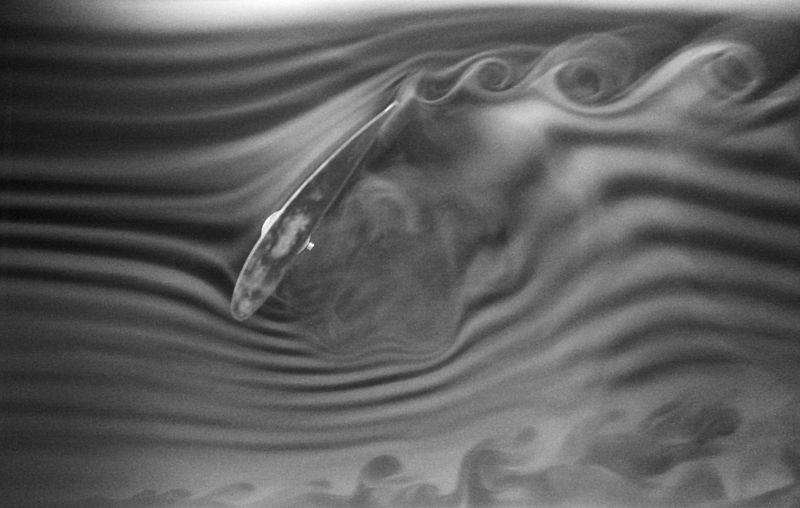
\includegraphics[width=0.5\textwidth]{WindTunnel.jpg}
  \end{center}
  \vspace{-20pt}
  \caption{\small{An airfoil in a fog wind tunnel (image from Wikimedia Commons, Smart Blade GmbH).}}
\end{figure}

\noindent \textbf{References} \\
The wind tunnel problem was based on a similar exercise in Linear Algebra and Its Applications, 4th Edition, by David C. Lay, Addison-Wesley, 2012.

 

%%%%%%%%%%%%%%%%%%%%%%%%%%%%%%%%%%%%%%%%%%%%%%%%%%%%%%%%%%%%%%%%
%%%%%%%%%%%%%%%%%%%%%%%%%%%%%%%%%%%%%%%%%%%%%%%%%%%%%%%%%%%%%%%%
%%%%%%%%%%%%%%%%%%%%%%%%%%%%%%%%%%%%%%%%%%%%%%%%%%%%%%%%%%%%%%%%
%%%%%%%%%%%%%%%%%%%%%%%%%%%%%%%%%%%%%%%%%%%%%%%%%%%%%%%%%%%%%%%%
% SOLUTIONS
\newpage
\section*{Solutions}

\begin{enumerate} 
% ~~~~~~~~~~~~~~~~~~~~~~~~~~~~~~~~~~~~~~~~~~~~~~~~~~~~~~~~~~~~~~~~~~~~~~~~~~~~~~~~~
\item
\begin{enumerate}
\item We can simplify the left-hand side of the equation by computing the determinant.
\begin{align*}
  \begin{vmatrix}
   3 &  2 &  0 \\
   1 &  x &  0 \\
   7 & -3 &  4 \\
  \end{vmatrix}
 &=
  3 \begin{vmatrix} x & 0 \\ -3 & 4 \end{vmatrix} -
  2 \begin{vmatrix} 1 & 0 \\ 7 & 4 \end{vmatrix} +
  0 \begin{vmatrix} 1 & x \\ 7 & -3 \end{vmatrix} \\
 &=
  3(4x - 0) - 2(4 - 0) + 0(-3 -7x) \\
 &=
  12x - 8
\end{align*}
Substituting this result yields the equation $12x - 8 = 4$, from which the 
solution $x = 1$ is easily recovered.
% -  -  -  -  -  -  -  -  -  -  -  -  -  -  -  -  -  -  -  -  -  -  -  -  -  -  -  -  -  -  
\item
Expand both determinants and rearrange the equation:
\begin{align*}
 (x)(4x) - (1)(4) &= (-x)(2x+8) - (-2)(2) \\
 4x^2 - 4 &= -2x^2 - 8x + 4 \\
 6x^2 + 8x - 8 &= 0 \\
 (6x - 4)(x + 2) &= 0
\end{align*}
Therefore the solutions are $x = 2/3$ and $x = -2$.
\end{enumerate}
% ~~~~~~~~~~~~~~~~~~~~~~~~~~~~~~~~~~~~~~~~~~~~~~~~~~~~~~~~~~~~~~~~~~~~~~~~~~~~~~~~~
\item 
Use row-reduction operations on the augmented matrices.
\begin{align}
 \begin{amatrix}{4}
  1 & 2 & 0 & 1 & 1 \\
  3 & -1 & 1 & 2 & 5 \\
  0 & 1 & 0 & 2 & 0 \\
  4 & 0 & 3 & 1 & 10
 \end{amatrix}&
 \nonumber \\
 \begin{amatrix}{4}
  1 & 2 & 0 & 1 & 1 \\
  0 & -7 & 1 & -1 & 2 \\
  0 & 1 & 0 & 2 & 0 \\
  0 & -8 & 3 & -3 & 6
 \end{amatrix}&
 \begin{array}{l}
  R_2 \leftarrow R_2 - 3R_1 \\ R_4 \leftarrow R_4 - 4R_1 
 \end{array}
 \nonumber \\
 \begin{amatrix}{4}
  1 & 2 & 0 & 1 & 1 \\
  0 & 0 & 1 & 13 & 2 \\
  0 & 1 & 0 & 2 & 0 \\
  0 & 0 & 3 & 13 & 6
 \end{amatrix}&
 \begin{array}{l}
  R_2 \leftarrow R_2 + 7R_3 \\ R_4 \leftarrow R_4 + 8R_3
 \end{array}
 \nonumber \\
 \begin{amatrix}{4}
  1 & 2 & 0 & 1 & 1 \\
  0 & 0 & 1 & 13 & 2 \\
  0 & 1 & 0 & 2 & 0 \\
  0 & 0 & 0 & -26 & 0
 \end{amatrix}&
 \begin{array}{l}
  R_4 \leftarrow R_4 - 3R_2
 \end{array}
 \nonumber
\end{align}

This is equivalent to the system of equations

\begin{align}
 x + 2y + w &= 1 \nonumber \\
 z + 13w &= 2 \nonumber \\
 y + 2w &= 0 \label{q2_a:a} \\
 -26w &= 0 \label{q2_a:b}
\end{align}

Equations (\ref{q2_a:a}) and (\ref{q2_a:b}) show that $w = 0$ and
$y = 0$, and substitution yields $z = 2$ and $x = 1$.

% ~~~~~~~~~~~~~~~~~~~~~~~~~~~~~~~~~~~~~~~~~~~~~~~~~~~~~~~~~~~~~~~~~~~~~~~~~~~~~~~~~
\item
\BEN
\item
It's not possible to calculate the determinant of $A$, because $A$ is not square. We can however solve $A\mathbf{x}=\mathbf{b}$ for \textbf{x} using row operations:
\begin{align}
 \begin{amatrix}{4}
  -3 &  1 & 2 &  4 & 1 \\
   2 & -1 & 2 &  3 & 1 \\
   1 &  0 & 4 & -2 & 1
 \end{amatrix}&
 \nonumber \\
 \begin{amatrix}{4}
  0 &  1 & 14 & -2 &  4 \\
  0 & -1 & -6 &  7 & -1 \\
  1 &  0 &  4 & -2 &  1
 \end{amatrix}&
 \begin{array}{l}
  R_1 \leftarrow R_1 + 3R_3 \\ R_2 \leftarrow R_2 - 2R_3
 \end{array}
 \nonumber \\
 \begin{amatrix}{4}
  0 & 1 & 14 & -2 & 4 \\
  0 & 0 &  8 &  5 & 3 \\
  1 & 0 &  4 & -2 & 1
 \end{amatrix}&
 \begin{array}{l}
  R_2 \leftarrow R_2 + R_1
 \end{array}
 \nonumber
\end{align}

This is equivalent to the system of equations

\begin{align}
 y + 14z -2w &= 4 \label{asdfasdf} \\
 8z + 5w &= 3 \label{qwerqwer} \\
 x + 4z -2w &= 1 \label{zxcvzxcv}
\end{align}

Since there are fewer equations than unknowns we will parameterize the 
solution set by setting $w = t$, where $t$ is any real number.  From equation 
(\ref{qwerqwer}) we get $z = \frac{3}{8} - \frac{5}{8}t$.  Substituting $z$ into 
equations (\ref{zxcvzxcv}) and (\ref{asdfasdf}) yields $x = -\frac{1}{2} + 
\frac{9}{2}t$ and $y = -\frac{5}{4} + \frac{43}{4}t$. \\

Because of the free parameter $t$, there are infinitely many solutions to the given system.
% ~  ~  ~  ~  ~  ~  ~  ~  ~  ~  ~  ~  ~  ~  ~  ~  ~  ~  ~  ~  ~  ~  ~  ~  ~  ~  ~  ~  ~  ~  ~  ~  ~  ~  ~  ~  
\item
We can calculate the 3$\times$3 determinant by expanding into 2$\times$2 determinants:
\begin{align*}
 \begin{vmatrix}
  1 &  2 & -1 \\
  2 &  5 &  0 \\
 4 & 9 &  -2
 \end{vmatrix} &=
 1 \begin{vmatrix} 5 & 0 \\ 9 & -2 \end{vmatrix}
 -2 \begin{vmatrix} 2 & 0 \\ 4 & -2 \end{vmatrix}
 -1 \begin{vmatrix} 2 & 5 \\ 4 & 9 \end{vmatrix} \\
 &= (-10) -2 (-4) -(18 - 20) \\
 &= -10 + 8 + 2 \\
 &= 0
\end{align*}
Applying one row operation yields
\begin{align*}
 \begin{amatrix}{3}
  1 & 2 & -1  & 1 \\
  2 & 5 & 0 & 5 \\
  4 & 9 & -2 & 0 
 \end{amatrix} \\
  \begin{amatrix}{3}
  1 & 2 & -1  & 1 \\
  2 & 5 & 0 & 5 \\
  4 & 9 & -2 & 0 
 \end{amatrix}
 \end{align*}
 
 % ~~~~~~~~~~~~~~~~~~~~~~~~~~~~~~~~~~~~~~~~~~~~~~~~~~~~~~~~~~~~~~~~~~~~~~~~~~~~~~~~~
\EEN

\item The derivative of $\textbf{r}$ is simply
\(
  \mathbf{r}'(t) = 2t \mathbf{i} + \mathbf{j}.
\)
Thus,
\BEN
\item \(
  \mathbf{r}(t) \perp  \mathbf{r}'(t)
\)
implies
\begin{align*}
  0& = \mathbf{r}(t) \cdot  \mathbf{r}'(t) \\
  &= \big((1+t^2) \mathbf{i} + t\mathbf{j} \big) \cdot \big(2t \mathbf{i} + \mathbf{j}\big) \\
  &= (2t+2t^3) + (t)\\
  &= t(3+2t^2)
\end{align*}
This equation is satisfied only when $t=0$ or $t^2 = -3/2$. The latter equation cannot be satisfied if $t\in\R$. Thus, the two vectors are only perpendicular when $t=0$. Thus,  \(\mathbf{r}(t)\) is perpendicular to \(\mathbf{r}'(t)\) at (0,1). 
\item If \(\mathbf{r}(t)\) is pointing in the same direction as \(\mathbf{r}'(t)\), then \(\mathbf{r}(t) \parallel  \mathbf{r}'(t)\), and 
\EEN
\end{enumerate} % END OF SOLUTIONS

\subsection*{Question ?}

We first convert the system of equations into an equivalent augmented-matrix
form:
\[
 \begin{amatrix}{3}
  1 & 2 & -1 & 2 \\
  2 & a & -2 & b \\
  3 & 2 & 0 & 1
 \end{amatrix}.
\]
Then apply a sequence of row-reduction operations:
\begin{align}
 \begin{amatrix}{3}
  1 &   2 & -1 &   2 \\
  0 & a-4 &  0 & b-4 \\
  0 &  -4 &  3 &  -5
 \end{amatrix} &  \nonumber \\
 \begin{amatrix}{3}
  1 &  2 & -1 &   2 \\
  0 &  a & -3 & b+1 \\
  0 & -4 &  3 &  -5
 \end{amatrix} & \begin{array}{l} R_2 - 2R_1 \\ R_3 - 3R_1 \end{array} 
 \nonumber \\
 \begin{amatrix}{3}
  1 & 2 & -1 &   2 \\
  0 & a & -3 & b+1 \\
  0 & 4 & -3 &   5
 \end{amatrix} &  \begin{array}{l} R_2 - R_3 \end{array}
 \nonumber \\
 \begin{amatrix}{3}
  1 & 2 & -1 &   2 \\
  0 & 4 & -3 &   5 \\
  0 & a & -3 & b+1
 \end{amatrix} &\begin{array}{l} -1 \cdot R_3 \\ R_2 \leftrightarrow R_3 \end{array}
 \label{eq:reduced}
\end{align}

Suppose that $a = 4$.  Then (\ref{eq:reduced}) becomes
\begin{align}
 \begin{amatrix}{3}
  1 & 2 & -1 &   2 \\
  0 & 4 & -3 &   5 \\
  0 & 4 & -3 & b+1
 \end{amatrix} &
 \nonumber \\
 \begin{amatrix}{3}
  1 & 2 & -1 &   2 \\
  0 & 4 & -3 &   5 \\
  0 & 0 &  0 & b-4
 \end{amatrix}&  \begin{array}{l} R_3 - R_2 \end{array}
 \label{eq:substitute_a}
\end{align}

If $b \neq 4$, then the system has no solutions, since the last row is
equivalent to the equation $0 = b-4$ where $b-4 \neq 0$.  Conversely, if
$b = 4$, then (\ref{eq:substitute_a}) is equivalent to the system of
equations
\begin{align*}
 x + 2y -z &= 2 \\
 4y - 3z &= 5
\end{align*}
There are fewer equations than unknowns, so we have to parameterize the
solution set; let $z = t$.  Solving these two equations yields the solution
\begin{equation}\begin{aligned}
 x &= -\frac{1}{2} - \frac{1}{2}t \\
 y &= \frac{5}{4} + \frac{3}{4}t \\
 z &= t
\end{aligned}\label{q4:inf}\end{equation}

Now suppose that $a = 0$.  Then the matrix (\ref{eq:reduced}) is equivalent
to the system

\begin{align*}
 x + 2y -z &= 2 \\
 4y -3z &= 5 \\
 -3z &= b+1
\end{align*}

Using back-substitution we find that

\begin{equation}\begin{aligned}
 x &= -\frac{1}{3} - \frac{1}{6}b \\
 y &= 1 - \frac{1}{4}b \\
 z &= \frac{-1}{3} - \frac{1}{3}b
\end{aligned}\label{q4:a_zero}\end{equation}

Now suppose that $a \neq 4$ and $a \neq 0$.  Then we can continue row-
reducing from (\ref{eq:reduced}):

\begin{align}
 \begin{amatrix}{3}
  1 & 2 & -1 &   2 \\
  0 & 4 & -3 &   5 \\
  0 & a & -3 & b+1
 \end{amatrix} &
 \nonumber \\
 \begin{amatrix}{3}
  1 & 2 & -1 & 2 \\
  0 & 4 & -3 & 5 \\
  0 & 0 & -3 + \frac{3}{4}a & 1 + b - \frac{5}{4}a
 \end{amatrix}&
 \begin{array}{l}
  R_3 \leftarrow R_3 - \dfrac{a}{4}R_2
 \end{array} 
 \nonumber
\end{align}

This is equivalent to the system

\begin{align*}
 x + 2y - z &= 2 \\
 4y -3z &= 5 \\
 (-3 + \frac{3}{4}a)z &= 1 + b - \frac{5}{4}a
\end{align*}

Let $c = \dfrac{1 + b - \frac{5}{4}a}{-3 + \frac{3}{4}a}$.  Using back-substitution we find the solution

\begin{equation}\begin{aligned}
 x &= -\frac{1}{2} - \frac{1}{2}c \\
 y &= \frac{5}{4} + \frac{3}{4}c \\
 z &= c
\end{aligned}\label{q4:one}\end{equation}

Thus we have shown that:
\begin{enumerate}
\item When $a = 4$ and $b = 4$ there are infinitely many solutions, given
by the parameterization (\ref{q4:inf}).
\item When $a = 4$ and $b \neq 4$ there are no solutions.
\item When $a \neq 4$ there is one solution.  When $a = 0$, the 
solution (\ref{q4:a_zero}) is equivalent to that of (\ref{q4:one}).  
So the solution when $a \neq 4$ is given by (\ref{q4:one}).
\end{enumerate}
% ~~~~~~~~~~~~~~~~~~~~~~~~~~~~~~~~~~~~~~~~~~~~~~~~~~~~~~~~~~~~~~~~~~~~~~~~~~~~~~~~~

\subsection*{Question 7}
\subsubsection*{(a)}
We can write the system as
\begin{align*}
a_0+a_1(0)+a_2(0)^2 +a_3(0)^3 &= 0 \\
a_0+a_1(1)+a_2(1)^2 +a_3(1)^3 &= 5.5 \\
a_0+a_1(2)+a_2(2)^2 +a_3(2)^3&= 20  \\
a_0+a_1(3)+a_2(3)^2 +a_3(3)^3 &= 46.5 \\
a_0+a_1(4)+a_2(4)^2 +a_3(4)^3 &= 88 \\ 
\end{align*}
Equivalently, we can write this as
\begin{align*}
\BM
1 & 0 & 0 & 0 \\
1 & 1 &1 &1\\
1&2&4&8\\ 
1&3&9&27\\ 
1&4&16&64\\ 
 \EM
 \BM a_0\\a_1\\a_2\\a_3 \EM 
 =  \BM 0\\5.5\\20\\46.5\\88 \EM 
\end{align*}

\subsubsection*{(b)}
Solving the above system yields 
\begin{align*}
 \BM a_0\\a_1\\a_2\\a_3 \EM 
 =  \BM 0\\2\\3\\0.5 \EM 
\end{align*}
\subsubsection*{(c)}
$p(1.5) = 2(1.5)+3(1.5)^2+0.5(1.5)^3 = 11.4375$
\subsubsection*{(d)}
The system for a polynomial of lower order would have no solution because $a_3 \ne 0$. For example, if we used a linear function, the system becomes
\begin{align*}
\BM
1&0\\
1&1\\
1&2\\ 
1&3\\ 
1&4\\ 
 \EM
 \BM a_0\\a_1 \EM 
 =  \BM 0\\5.5\\20\\46.5\\88 \EM 
\end{align*}
This system has no solution. 

\end{document}


% QUESTIONS AND SOLUTIONS ON SIMILAR AND ORTHOGONAL MATRICES

%% -  -  -  -  -  -  -  -  -  -  -  -  -  -  -  -  -  -  -  -  -  -  -  -  -  -  -  -  -  -  
%\item 
%% QUESTION 5, MEDIUM
%%GPS: MMCA2c
%Let $A, B, C$ be three square matrices with the same dimensions.
%\begin{enumerate}
%\item Prove that if $A$ and $B$ are similar and $B$ and $C$ are similar then 
%$A$ and $C$ are similar.
%\item Let $x \in R$.  Prove that $A$ and $B + xI$ are similar whenever
%$A - xI$ and $B$ are similar.
%\item Suppose the system $A\mathbf{x} = \mathbf{b}$ has infinitely many solutions $x$ and that
%$A$ and $B$ are similar.  How many solutions can $B\mathbf{x} = \mathbf{b}$ have?
%\end{enumerate}
%
%% -  -  -  -  -  -  -  -  -  -  -  -  -  -  -  -  -  -  -  -  -  -  -  -  -  -  -  -  -  -  
%\item 
%% QUESTION 6, MEDIUM
%%GPS: MMCA2b 
%
%\begin{enumerate}
%\item Prove that, for any vectors $\mathbf{u}, \mathbf{v}$ and any orthogonal matrix $X$, $\mathbf{u} 
%\cdot \mathbf{v} = X\mathbf{u} \cdot X\mathbf{v}$
%\item Let $\mathbf{u}$ and $\mathbf{v}$ be two distinct vectors in $\R^{2}$.  Prove that, when 
%$X$ is an orthogonal matrix, the area of the parallelogram determined by $\mathbf{u}$ 
%and $\mathbf{v}$ is equal to the area of the parallelogram determined by $X\mathbf{u}$ and 
%$X\mathbf{v}$.
%\end{enumerate}

%
%\subsubsection*{(b)}
%
%Form the augmented matrix and apply row-reduction operations:
%
%\begin{align}
% \begin{bmatrix}
%  1 & 2 & -1 & 1 & 0 & 0 \\
%  2 & 5 & 0 & 0 & 1 & 0 \\
%  -3 & -5 & 4 & 0 & 0 & 1
% \end{bmatrix}&
% \nonumber \\
% \begin{bmatrix}
%  1 & 2 & -1 & 1 & 0 & 0 \\
%  0 & 1 & 2 & -2 & 1 & 0 \\
%  0 & 1 & 1 & 3 & 0 & 1
% \end{bmatrix}&
% \begin{array}{l}
%  R_2 \leftarrow R_2 - 2R_1 \\
%  R_3 \leftarrow R_3 + 3R_1
% \end{array}
% \nonumber \\
% \begin{bmatrix}
%  1 & 2 & -1 & 1 & 0 & 0 \\
%  0 & 1 & 2 & -2 & 1 & 0 \\
%  0 & 0 & -1 & 5 & -1 & 1
% \end{bmatrix}&
% \begin{array}{l}
%  R_3 \leftarrow R_3 - R_2
% \end{array}
% \nonumber \\
% \begin{bmatrix}
%  1 & 2 & -1 & 1 & 0 & 0 \\
%  0 & 1 & 0 & 8 & -1 & 2 \\
%  0 & 0 & 1 & -5 & 1 & -1
% \end{bmatrix}&
% \begin{array}{l}
%  R_2 \leftarrow R_2 + 2R_3 \\
%  R_3 \leftarrow -1 * R_3
% \end{array}
% \nonumber \\
% \begin{bmatrix}
%  1 & 0 & 0 & -20 & 3 & -5 \\
%  0 & 1 & 0 & 8 & -1 & 2 \\
%  0 & 0 & 1 & -5 & 1 & -1
% \end{bmatrix}&
% \begin{array}{l}
%  R_1 \leftarrow R_1 - 2R_2 + R_3
% \end{array}
% \nonumber
%\end{align}
%
%So the inverse matrix is
%\(\begin{bmatrix} -20 & 3 & -5 \\ 8 & -1 & 2 \\ -5 & 1 & -1 \end{bmatrix}\).
%
%\subsubsection*{(c)}
%
%The matrices $A_i$ are found by replacing the $i^{th}$ column of $A$ with
%the vector $b$.
%
%\begin{align*}
% A_1 &=
%  \begin{bmatrix}
%   1 & 2 & -1 \\
%   2 & 5 & 0 \\
%   -1 & -5 & 4
%  \end{bmatrix}, \det(A_1) = 20 - 16 + 5 = 9 \\
% A_2 &=
%  \begin{bmatrix}
%   1 & 1 & -1 \\
%   2 & 2 & 0 \\
%   -3 & -1 & 4
%  \end{bmatrix}, \det(A_2) = 8 - 8 - 4 = -4 \\
% A_3 &=
%  \begin{bmatrix}
%   1 & 2 & 1 \\
%   2 & 5 & 2 \\
%   -3 & -5 & -1
%  \end{bmatrix}, \det(A_3) = 5 - 8 + 5 = 2
%\end{align*}
%\subsection*{Question 5}
%
%\subsubsection*{(a)}
%Since $A$ and $B$ are similar and $B$ and $C$ are similar there exist
%matrices $S$ and $T$ such that $A = S^{-1}BS$ and $B = T^{-1}CT$; by
%substitution we see that $A = S^{-1}(T^{-1}CT)S = (TS)^{-1}C(TS)$.  If
%we set $U = TS$, then $A = U^{-1}CU$, so that A and C are similar.
%
%\subsubsection*{(b)}
%Since $A - xI$ and $B$ are similar there exists a square invertible matrix
%$C$ such that $C^{-1}(A - xI)C = B$.  By expanding the left-hand side of the
%equation we get $C^{-1}AC - C^{-1}xIC = B$.  However, since $x$ is a scalar,
%$C^{-1}xIC = xC^{-1}IC = xC^{-1}C = xI$, so that $C^{-1}AC - xI = B$.  By
%rearranging we see that $B + xI = C^{-1}AC$, so that $A$ and $B + xI$ are
%similar.
%
%\subsubsection*{(c)}
%Since $A$ and $B$ are similar, they have the same determinant.  The system
%$A\mathbf{x} = \mathbf{b}$ has infinitely many solutions, which, since $A$ is square, implies 
%that $A$ is not invertible, so that $\det(A) = \det(B) = 0$.  Therefore the 
%system $B\mathbf{x} = \mathbf{b}$ is either unsolvable or has infinitely many solutions.
%
%\subsection*{Question 6}
%
%\subsubsection*{(a)}
%Since $\mathbf{u} \cdot \mathbf{v} = \mathbf{u}^{T}\mathbf{v}$ for any vectors $\mathbf{u}, \mathbf{v}$ and $X^{T}X = I$, $X\mathbf{u}
%\cdot X\mathbf{v} = (X\mathbf{u})^{T}X\mathbf{v} = \mathbf{u}^{T}X^{T}X\mathbf{v} = \mathbf{u}^{T}\mathbf{v} = \mathbf{u} \cdot \mathbf{v}$.
%
%\subsubsection*{(b)}
%The area $area_{\mathbf{u},\mathbf{v}}$ of the parallelogram determined by $\mathbf{u}$ and $\mathbf{v}$ is given by the magnitude of the cross product $\mathbf{u} \times \mathbf{v}$:
%\[area_{\mathbf{u},\mathbf{v}} = ||\mathbf{u}||||\mathbf{v}|| \cdot |\sin(\theta_{\mathbf{u},\mathbf{v}})|\]
%where $\theta_{\mathbf{u},\mathbf{v}}$ is the angle between the vectors $\mathbf{u}, \mathbf{v}$.  Similarly,
%\[area_{X\mathbf{u},X\mathbf{v}}\ = ||X\mathbf{u}||||X\mathbf{v}|| \cdot |\sin(\theta_{X\mathbf{u},X\mathbf{v}})|\]
%Applying part (a) we see that $||X\mathbf{u}|| = \sqrt{X\mathbf{u} \cdot X\mathbf{u}} = \sqrt{\mathbf{u} \cdot \mathbf{u}} = ||\mathbf{u}||$ and $||X\mathbf{v}|| = ||\mathbf{v}||$.  Additionally,
%\begin{align*}
% \sin(\theta_{X\mathbf{u},X\mathbf{v}}) &= \sqrt{1 - \cos(\theta_{X\mathbf{u},X\mathbf{v}})^{2}} \\
% & = \sqrt{1 - (\dfrac{X\mathbf{u} \cdot X\mathbf{v}}{||X\mathbf{u}||||X\mathbf{v}||})^{2}} \\
% &= \sqrt{1 - (\dfrac{\mathbf{u} \cdot \mathbf{v}}{||\mathbf{u}||||\mathbf{v}||})^{2}} \\
% &= \sqrt{1 - \cos(\theta_{\mathbf{u},\mathbf{v}})^{2}} \\
% &= |\sin(\theta_{\mathbf{u},\mathbf{v}})|.
%\end{align*}
%
%Thus $area_{X\mathbf{u},X\mathbf{v}} = area_{\mathbf{u},\mathbf{v}}$.

